\documentclass{article} 
\usepackage[pdftex]{epsfig}
\usepackage{fancyhdr,subfig,graphicx,psfrag,amsfonts,mathtools,amsmath,hyperref} 
\usepackage[margin=1.5cm]{geometry}

\title{Mandatory exercise 3 \\
Signal and Image Processing 2012} 
\author{Jens P. Raaby \\
\url{frn617@diku.dk}}

\begin{document} 
\maketitle

\section*{Question 3.1 - Noisy Signals}
Generating a 100 element vector of samples according to a given noise type was relatively easy with Matlab, with the exception of the Salt and Pepper noise which took some time to understand correctly. 

The file noiseGen1D.m contains a function to generate such samples. The histograms of the samples generated are shown in figure \ref{fig:q1} in the appendix. These and the parameter estimations are generated in the file q1.m.

In general, fitting parameters to a distribution will be more accurate with more samples. Therefore some of the inaccuracy of any estimates can be explained by the relatively small sample size.

\subsection*{Gaussian}
The Gaussian noise is generated using either of the functions randn and normrnd in MATLAB. It is relatively easy to estimate the parameters of the noisy signal, since they are defined:
\[
\mu = mean(sample)
\]
\[
\sigma = \sqrt{variance(sample)}
\]
Using these equations, I estimated the parameters at $\mu = -0.0528$ and $\sigma = 0.4758$.

\subsection*{Gamma}
Gamma noise parameters are slightly more complex to retrieve, but are still based on the mean and variance (equations 5.2-6 and 5.2-7 in Gonzalez \& Woods). With simple algebraic manipulation the terms $a$ and $b$ can be determined from the variance and mean:
%\begin{equation}
%\begin{array}{rl}
\[
a =  \frac {\mu} {\sigma ^2}
\]
\[
b =  \frac { \mu ^2} {\sigma ^2}
\]
%\end{array}
%\end{equation}
I found in practice that this returned some incorrect results (by testing different parameter values and comparing the estimates with those provided by Matlab's built in fitdist function). However for the given parameters (1,1) the error was not so great. I calculated $a=1.0343$ and $b=1.0801$.

\subsection*{Uniform}
In a similar manner to Gamma noise above, I rearranged the equations from Gonzalez and Woods to give:
\begin{equation}
\begin{array}{rl}
b = & \mu + \frac 1 2 {\sqrt{12\sigma ^2}}\\\\
a = & 2 \mu - b
\end{array}
\end{equation}
The results were quite accurate on the test data, giving $a=0.0667$ and $b=2.0825$.


\subsection*{Salt and pepper}
There was a lot of confusion and time wasting about this part of the assignment. Google did not help! 
My understanding of salt and pepper noise after reading more carefully (in particular the lecture slides provided at \url{http://cronos.rutgers.edu/~lrr/dsp\%20design\%20course/lectures/Lecture_IP5_2009.pdf}) is as follows:
The noise contains pepper (with intensity $a$)  with probability $P_a$, and salt (intensity $b$) with probability $P_b$. All other samples take some other value (with probability $1-(P_a + P_b)$). The original probabilities 0.1 and 0.2 made sense - 10\% of the signal should be pepper noise, and 20\% should be salt noise. The updated assignment changed the probabilities so that they sum to 1 (this is unnecessary, and means that the entire signal is noise!). 

Estimating the parameters is relatively easy when visually inspecting the histogram (see figure \ref{fig1:sandp}): there are two peaks at value 0 and 2, where one peak is twice the height of the other.

Calculating the parameters from the samples using the histogram (binned to the same size as the vector of samples) gave the following estimates:
$a = 0.0100$, $b = 1.9900$, $p_a = 0.3800$,$p_b =  0.6200$. These are close to the input parameters.

\subsection*{Using estimation with real images}
If the noise parameters of real images could be estimated using methods such as those I used above, it may be easier to restore the image to a less noisy condition. For example, if the salt and pepper noise parameters are estimated it should be relatively straightforward to replace the offending pixels (those with intensities $a$ and $b$) with the mean of the pixel neighbourhoods.
In the other types of noise, the pattern is more complex and (being stochastic) quite difficult to eliminate completely from inaccurate estimates. I would expect that using an iterative algorithm might be able to help in this instance. Once a basic estimate of noise parameters is known, subtract a m x n copy of the noise from the image (where the image size is m x n). Inspect the noise of the resulting image, and change each parameter in turn while observing the effect. If there is an improvement (reduction), keep adjusting the parameter in the same way until no improvements are observed. This 'gradient descent' approach would not be particularly practical in many cases.
A better approach would be to isolate a part of the image with relatively little detail (so that it is harder to confuse desirable pixels with noise) and estimate the noise parameters for only that area. Then one could use the parameters to tweak a noise removal filter.
 According to Gonzalez and Woods, various spatial filters  (such as mean) are typically used to smooth away noise from images. The order-statistic filters should yield even better results (for example the median filter mentioned in GW section 5.3.2).


\section*{Question 3.2 - Filtering out Noise}

\subsection*{house.tif}
Inspecting the histogram reveals what appears to be 2 spikes, suggesting salt and pepper noise. I used the imhist function to inspect the histogram and identified the pepper having value 6, and the salt having value 180. I tried using the wiener2 function, but as the noise is not so even (and constant power as the documentation states) the result was still peppery.
According to Gonzalez and Woods section 5.3.1, the contra harmonic mean filter is well suited to removing salt and pepper noise. I implemented this filter using Matlab's built in imfilter function. Figure \ref{q2:house} shows the results.
\begin{figure}[h]
\subfloat[Original image]{\label{fig2:house}\includegraphics[width=0.3\textwidth]{q2-house.png}}\qquad
\subfloat[Pepper removed ($Q = 1.5$, $3x3$ mask)]{\label{fig2:housepep}\includegraphics[width=0.3\textwidth]{q2-depeppered.png}}\qquad
\subfloat[Salt removed ($Q = -10$, $3x3$ mask)]{\label{fig2:housesalt}\includegraphics[width=0.3\textwidth]{q2-desalted.png}}
\caption{Applying the contra harmonic filter to house.tif}
\label{q2:house}
\end{figure}
The main problem with this filtering was that the two successive filterings reduced detail from the original image. The first filter ($Q=1.5$) increased blur in the darker areas (on the walls) thus spreading the salt noise. The second filter removed a lot of the salt but left some behind (thanks to the earlier blurring) and it also blurred the lighter areas. The final result is less sharp but cleaner at low magnification.

\subsection*{ic.tif}
This image has narrow dynamic range and a lot of fairly even looking noise. Inspecting the histogram in figure \ref{fig2:ichist} shows a shape that appears to have a Gaussian distribution.  Therefore the wiener2 function should be a better fit for this image. It looks at the neighbourhood for each pixel and adaptively removes noise. The result is shown (figure \ref{fig2:icwiener}) along with the histogram (figure \ref{fig2:icwhist}). There was not very much detail in the original image so the larger mask could be used to remove more noise.
\begin{figure}[h]
\subfloat[Original image]{\label{fig2:ic}\includegraphics[width=0.22\textwidth]{q2-ic.png}}\qquad
\subfloat[Result of wiener2 function (15x15 mask)]{\label{fig2:icwiener}\includegraphics[width=0.22\textwidth]{q2-icwienered.png}}\qquad
\subfloat[Original histogram]{\label{fig2:ichist}\includegraphics[width=0.22\textwidth]{q2-ichist.pdf}}
\subfloat[Histogram after filtering]{\label{fig2:icwhist}\includegraphics[width=0.22\textwidth]{q2-icwieneredhist.pdf}}
\caption{Applying the wiener2 function to ic.tif}
\label{q2:ic}
\end{figure}

\subsection*{boxes.tif}
This image's histogram suggests 2 kinds of noise: salt and pepper (in this case with only salt) and Gaussian. The salt noise is at the maximum frequency. I therefore decided to apply a combination of the contra harmonic filter for removing the salt noise and the wiener2 function for the Gaussian noise. I tried applying them in both orders, and found that removing the Gaussian noise first yielded better results. This is because the contra harmonic filter with negative power Q blurs the other noise in the lighter regions. The result (figure \ref{fig2:boxwienerch}) is not perfectly sharp but a vast improvement over the original.
\begin{figure}[h]
\subfloat[Original image]{\label{fig2:boxes}\includegraphics[width=0.3\textwidth]{q2-boxes.png}}\qquad
\subfloat[Result of wiener2 function (3x3 mask)]{\label{fig2:boxwiener}\includegraphics[width=0.3\textwidth]{q2-boxes-wienered.png}}\qquad
\subfloat[Result of contra harmonic function (3x3 mask, $Q=-10$) applied to figure \ref{fig2:boxwiener}]{\label{fig2:boxwienerch}\includegraphics[width=0.3\textwidth]{q2-boxesdesalt.png}}\qquad
%\subfloat[Original histogram]{\label{fig2:boxhist}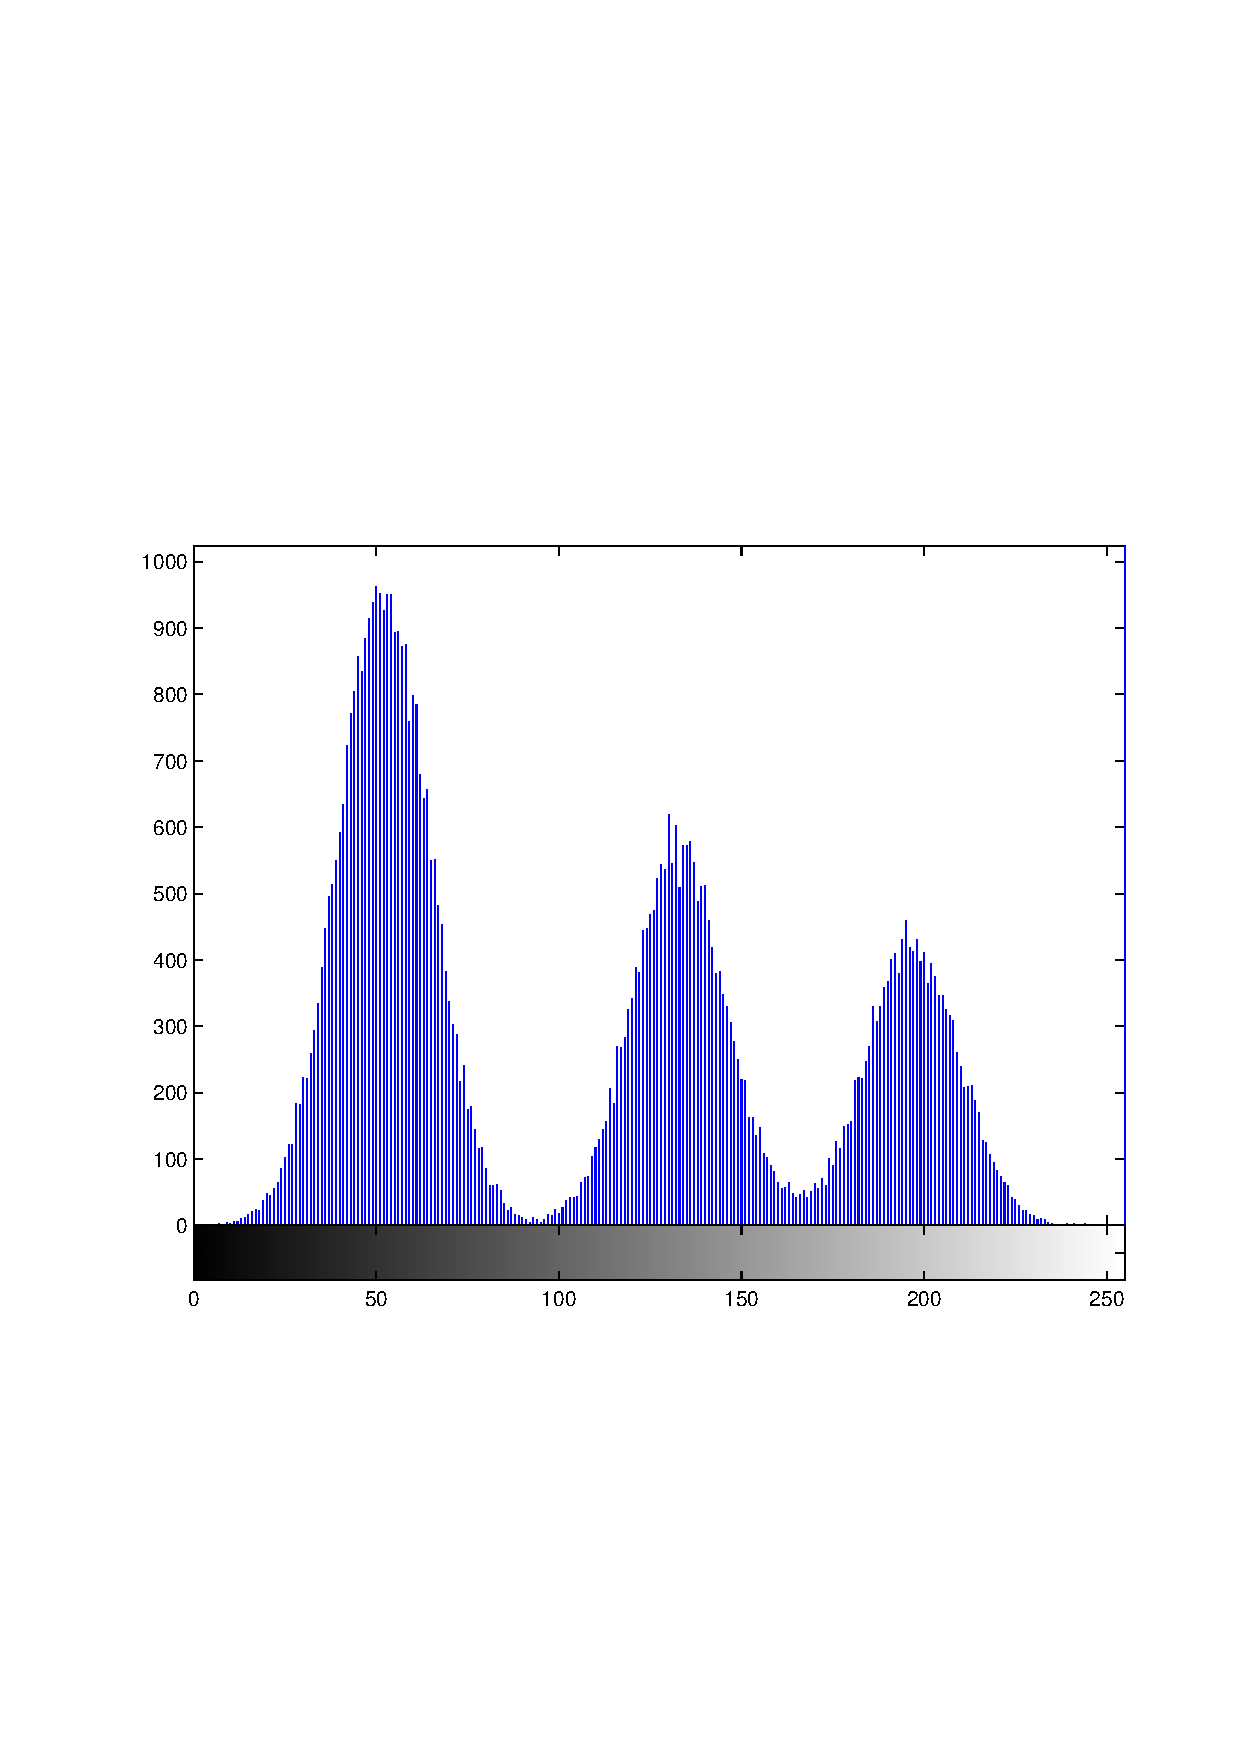
\includegraphics[width=0.4\textwidth]{q2-boxhist.pdf}}
%\subfloat[Histogram after filtering]{\label{fig2:boxfinalhist}\includegraphics[width=0.4\textwidth]{q2-boxhist-after.pdf}}
\caption{Applying the wiener2 function to boxes.tif}
\label{q2:boxes}
\end{figure}

\section*{Question 3.3 - Long exposure blurring}

\section*{Question 3.4 - Restoration}
\break
\appendix
\section{Figures}

\begin{figure}

\subfloat[Gaussian samples ($\mu = 0$, $\sigma = 0.5$)]{\label{fig1:gauss}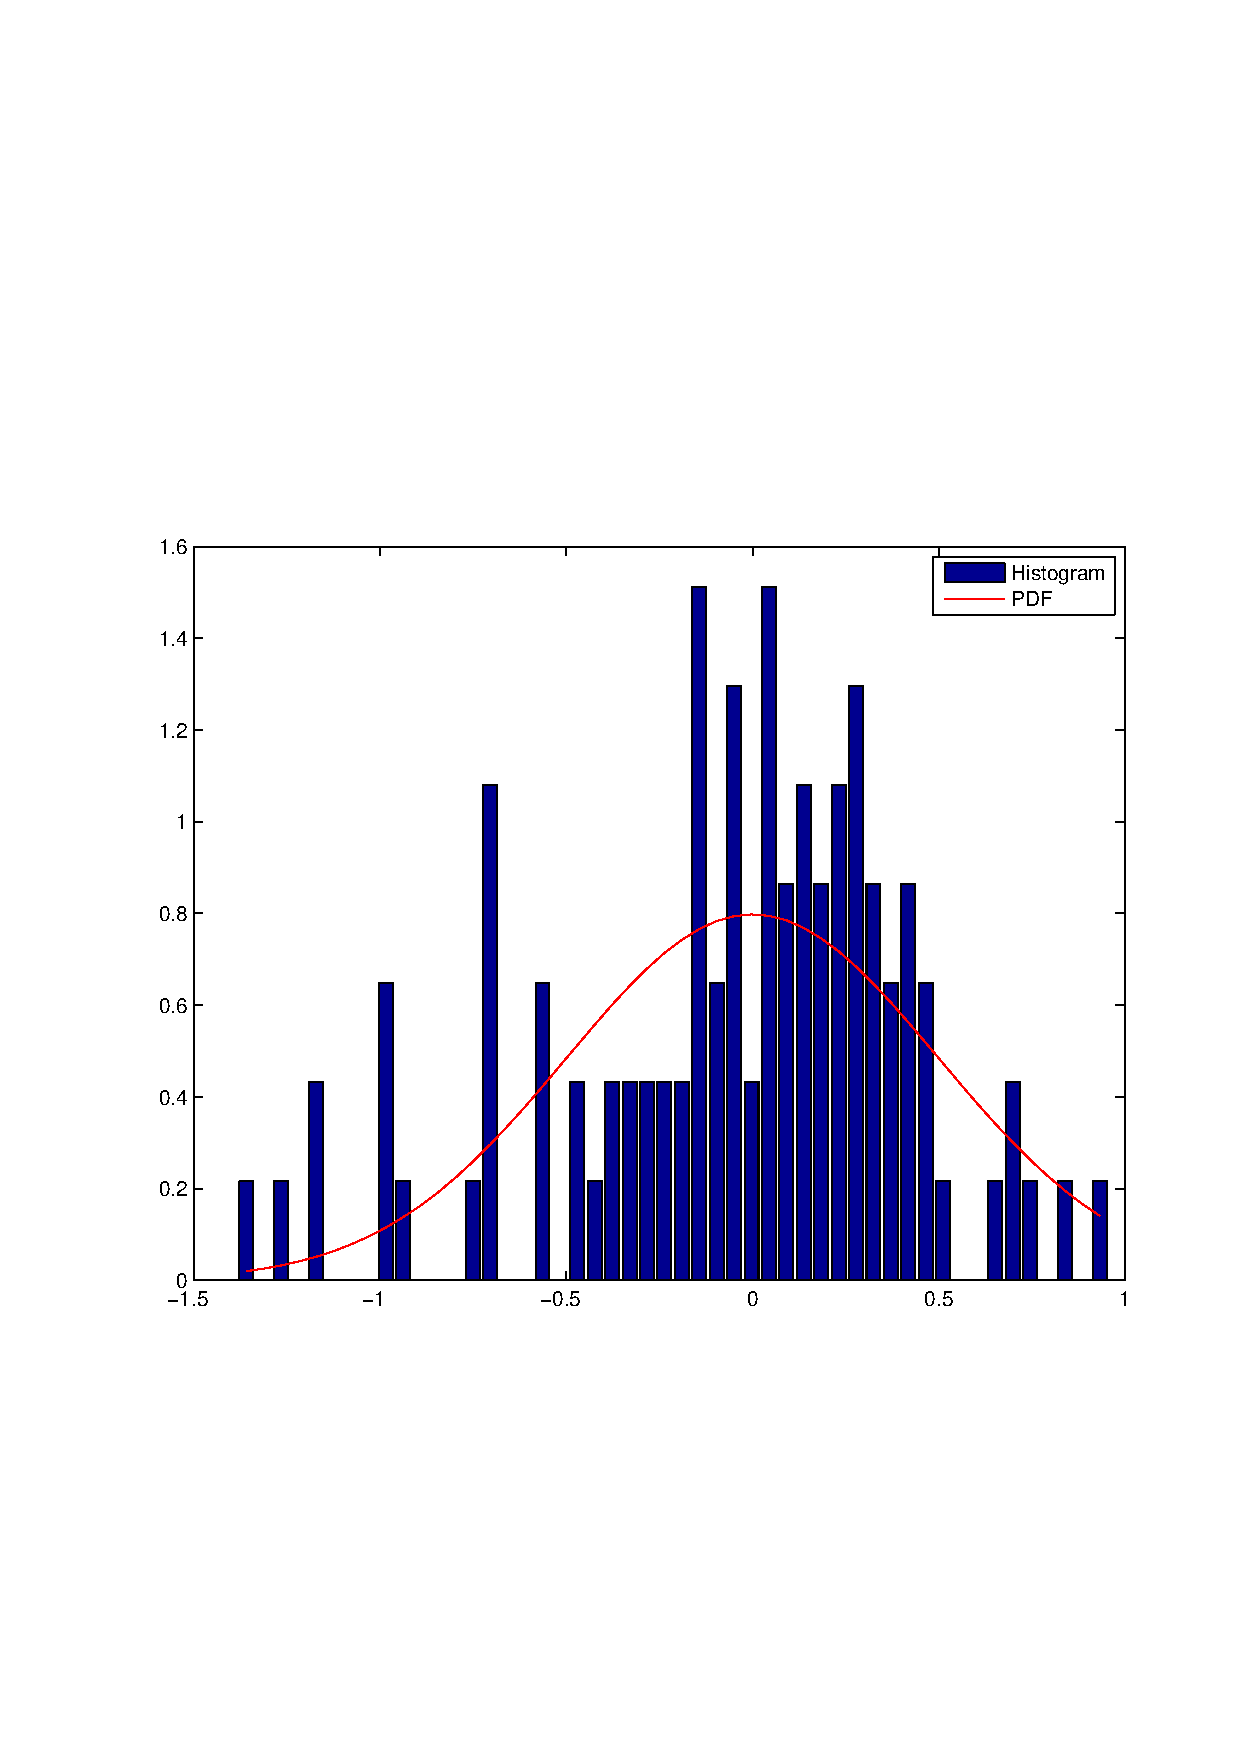
\includegraphics[width=0.5\textwidth]{q1-gaussian.pdf}}
\subfloat[Gamma samples ($a = 1$, $b = 1$)]{\label{fig1:gamma}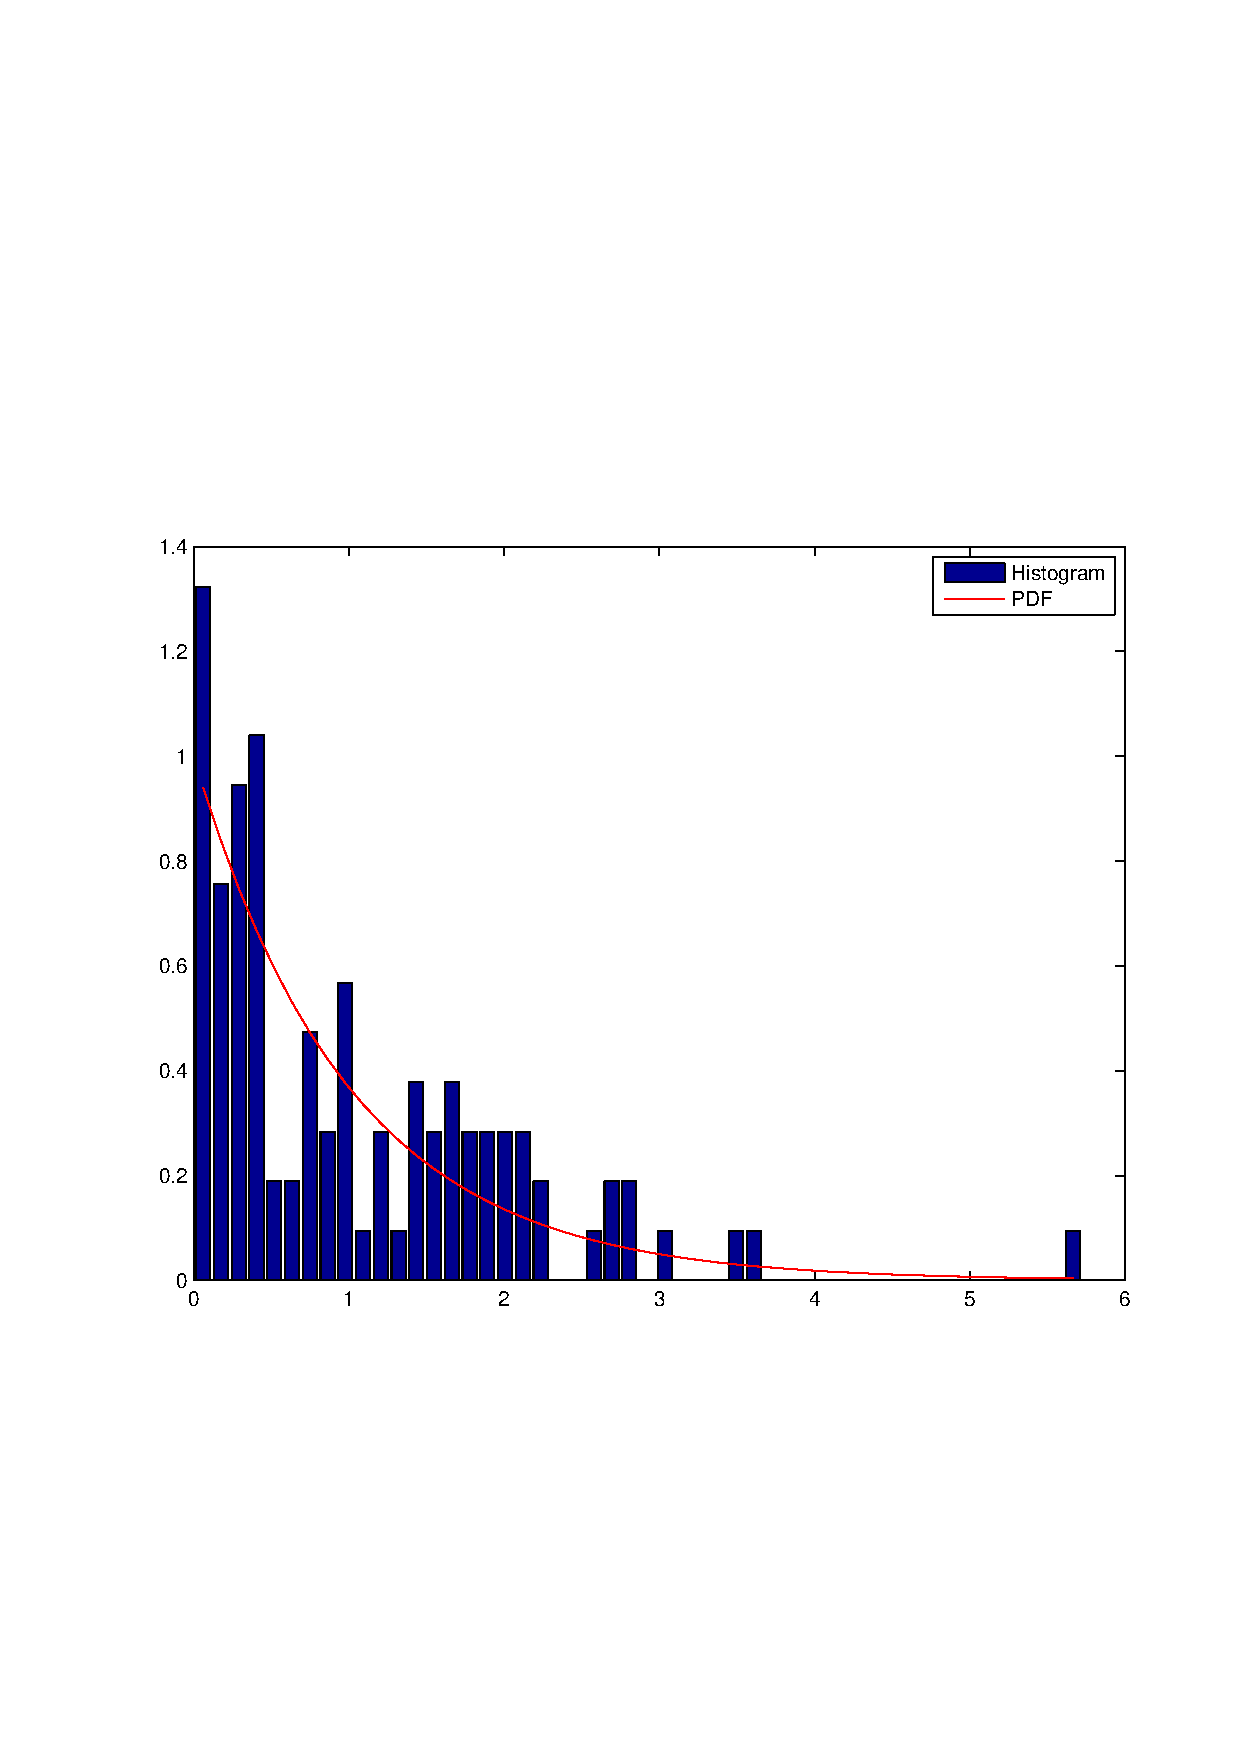
\includegraphics[width=0.5\textwidth]{q1-gamma.pdf}}\\
\subfloat[Uniform samples ($a = 0$, $b = 2$)]{\label{fig1:uniform}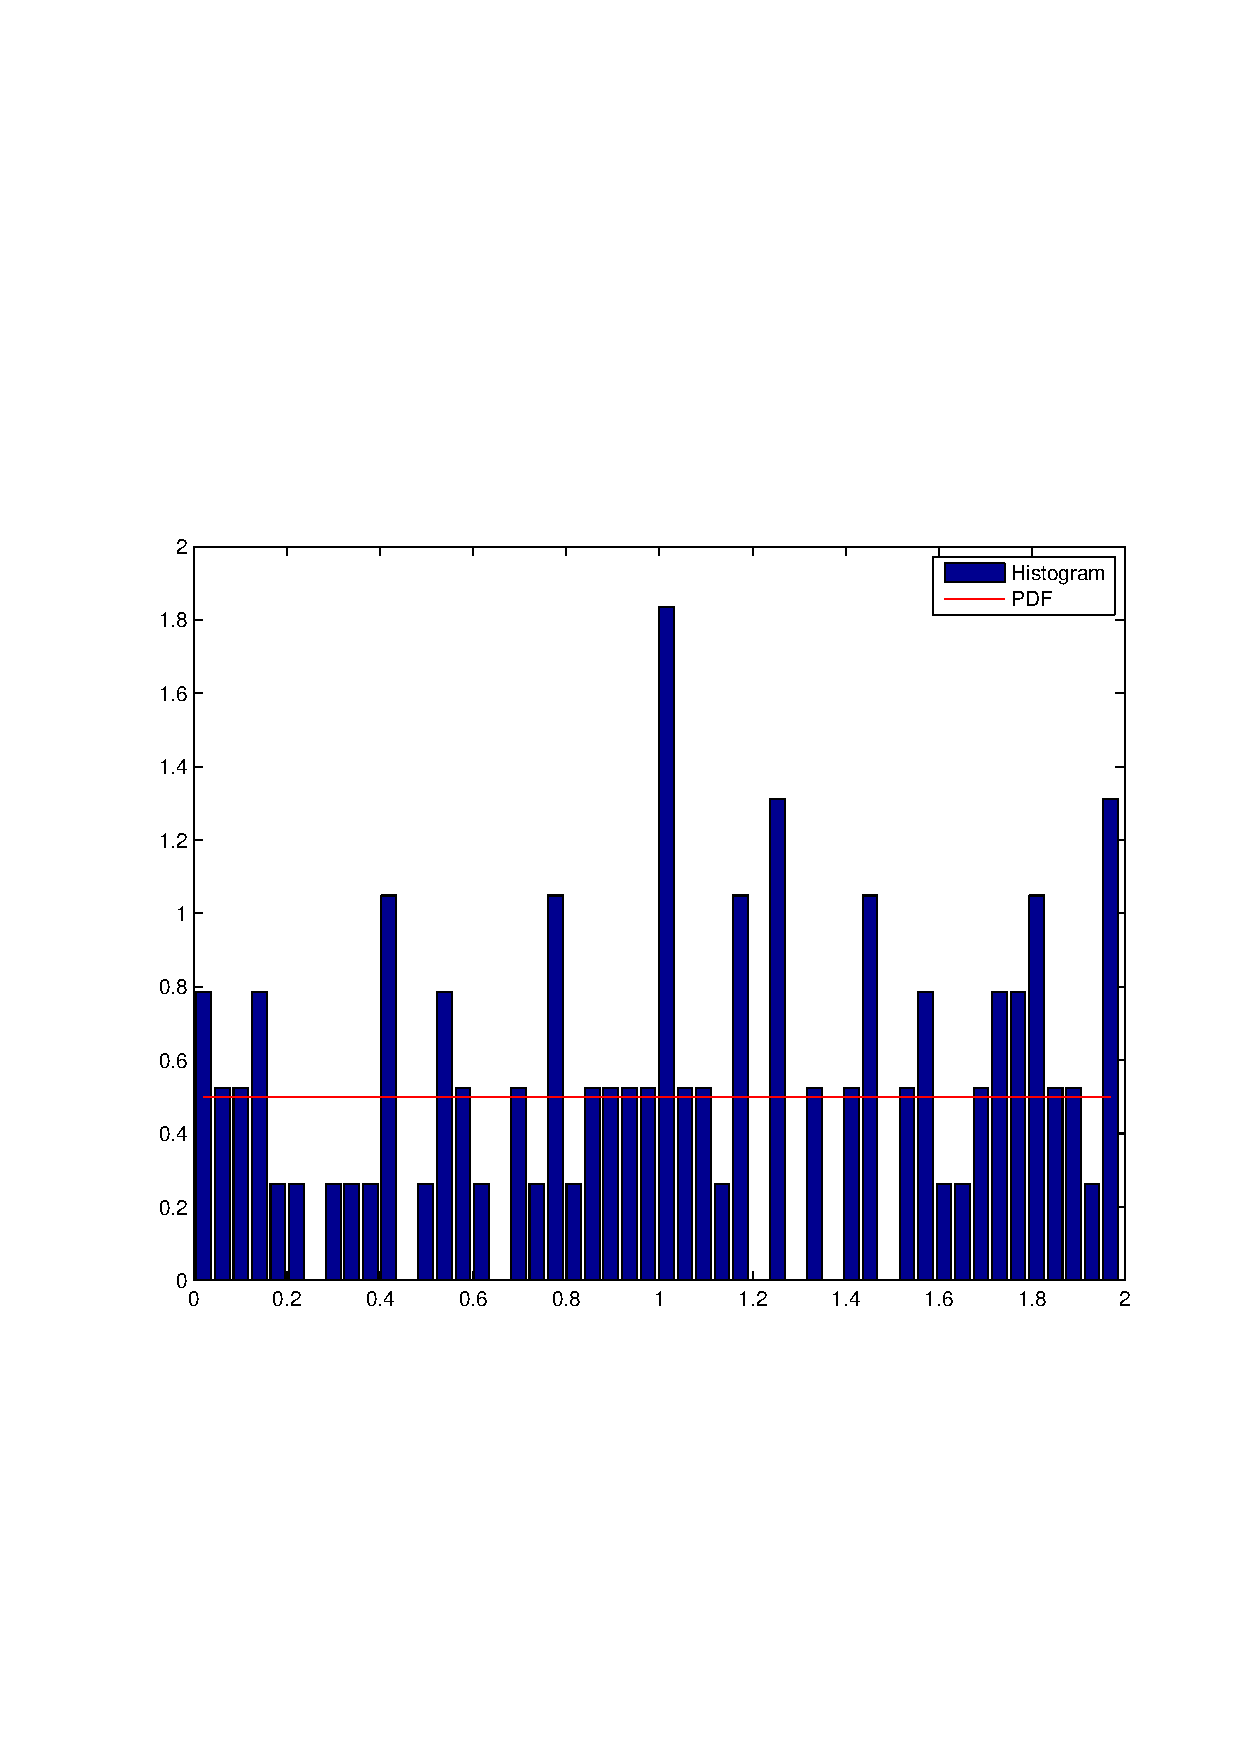
\includegraphics[width=0.5\textwidth]{q1-uniform.pdf}}
\subfloat[Salt \& Pepper samples ($P_0 = 1/3$, $P_2 = 2/3$)]{\label{fig1:sandp}\includegraphics[width=0.5\textwidth]{q1-sandp.pdf}}

\caption{Histograms for noise samples}
\label{fig:q1}
\end{figure}

 \end{document}
